\documentclass{article}[14pt]
\usepackage{amsmath}
\usepackage{amsfonts}
\usepackage{graphicx}
\usepackage{enumerate}
\usepackage{dtklogos}
\usepackage{verbatim}
\usepackage{amsmath}
\usepackage{listings}
\usepackage{url}
\usepackage{natbib}
\usepackage{calrsfs}
\usepackage{collectbox}
\usepackage{blindtext}
\newcommand{\R}{{\mathbb R}}
\renewcommand{\vec}[1]{{\mathbf #1}}
\newcommand{\points}[1]{\phantom{.}\hfill \textbf{(#1 points)}}
\newcommand{\matlab}{{\textsc{Matlab}} }


\begin{document}
\begin{center}


\title{Project 1}
\hfill Iliass Tiendrebeogo\\

\hfill \today\\
\end{center}
\bigskip

\begin{center}
  \begin{Large}
      
    Project $N^o 1$ \\
    Math 567: Winter 2016 \\
       
  \end{Large}
\end{center}

\bigskip

\begin{section}
%\item % GOP Nat Primary
{\bf \large 2016 National Republican Primary}

\begin{enumerate}[]

\item % The chart

This is the graphic of 2016 GOP Primary from Feb. 2015. Trends are as follow: we have Donald Trump's trend in red curve, Ben Carson's  in orange curve, Ted Cruz's in green curve, Marco Rubio's show in purple.

A quick view of the chart we can see that there are around six candidates which are still running and only three of them are  relevant. A more in depth analysis show that Donald Trump is leading the race although he got into the race late(April 2015).  He remain unknown during the first two months, before gaining  popularity at a very fast pace and keep growing until now with   $37\%$. Whereas, Ben Carson  had lead the second place with a growing popularity from August  to November where his popularity attain a pick at $ 20 \%$ and then drop bellow 10 for some reasons. And Ted Cruz,, who has his popularity below $10 \%$ flat since Feb. 2015 have started growing in popularity since November 2015, which might be cause by Ben Carson's falling and Republican need a second runner to trust. The others runners have had a pretty flat popularity which evolve around an average of $10\%$.

One important thing to notice is that lot of Republican Candidates haven't drop out yet.

\item {\bf \large The Script}


\end{enumerate}

\end{section}

\bigskip
\begin{section}
%\item % Dem National Primary
{ \bf \large 2016 National Democratic  Primary} 
\bigskip
\end{section}

\begin{section}
%\item % SC GOP
{\bf \large 2016 South Carolina Republican Presidential Primary}
\bigskip
\end{section}

\begin{section}
%\item % Obama's Job approval
{\bf \large President Obama's Job Approval}
\begin{enumerate}[]
\item {}


The Chart bellow of Obama's job approval since the start of his Presidency shows in red the approval rate, in green the disapproval rate from late 2008 to February 2016.

\begin{figure}[htb]
\begin{center}
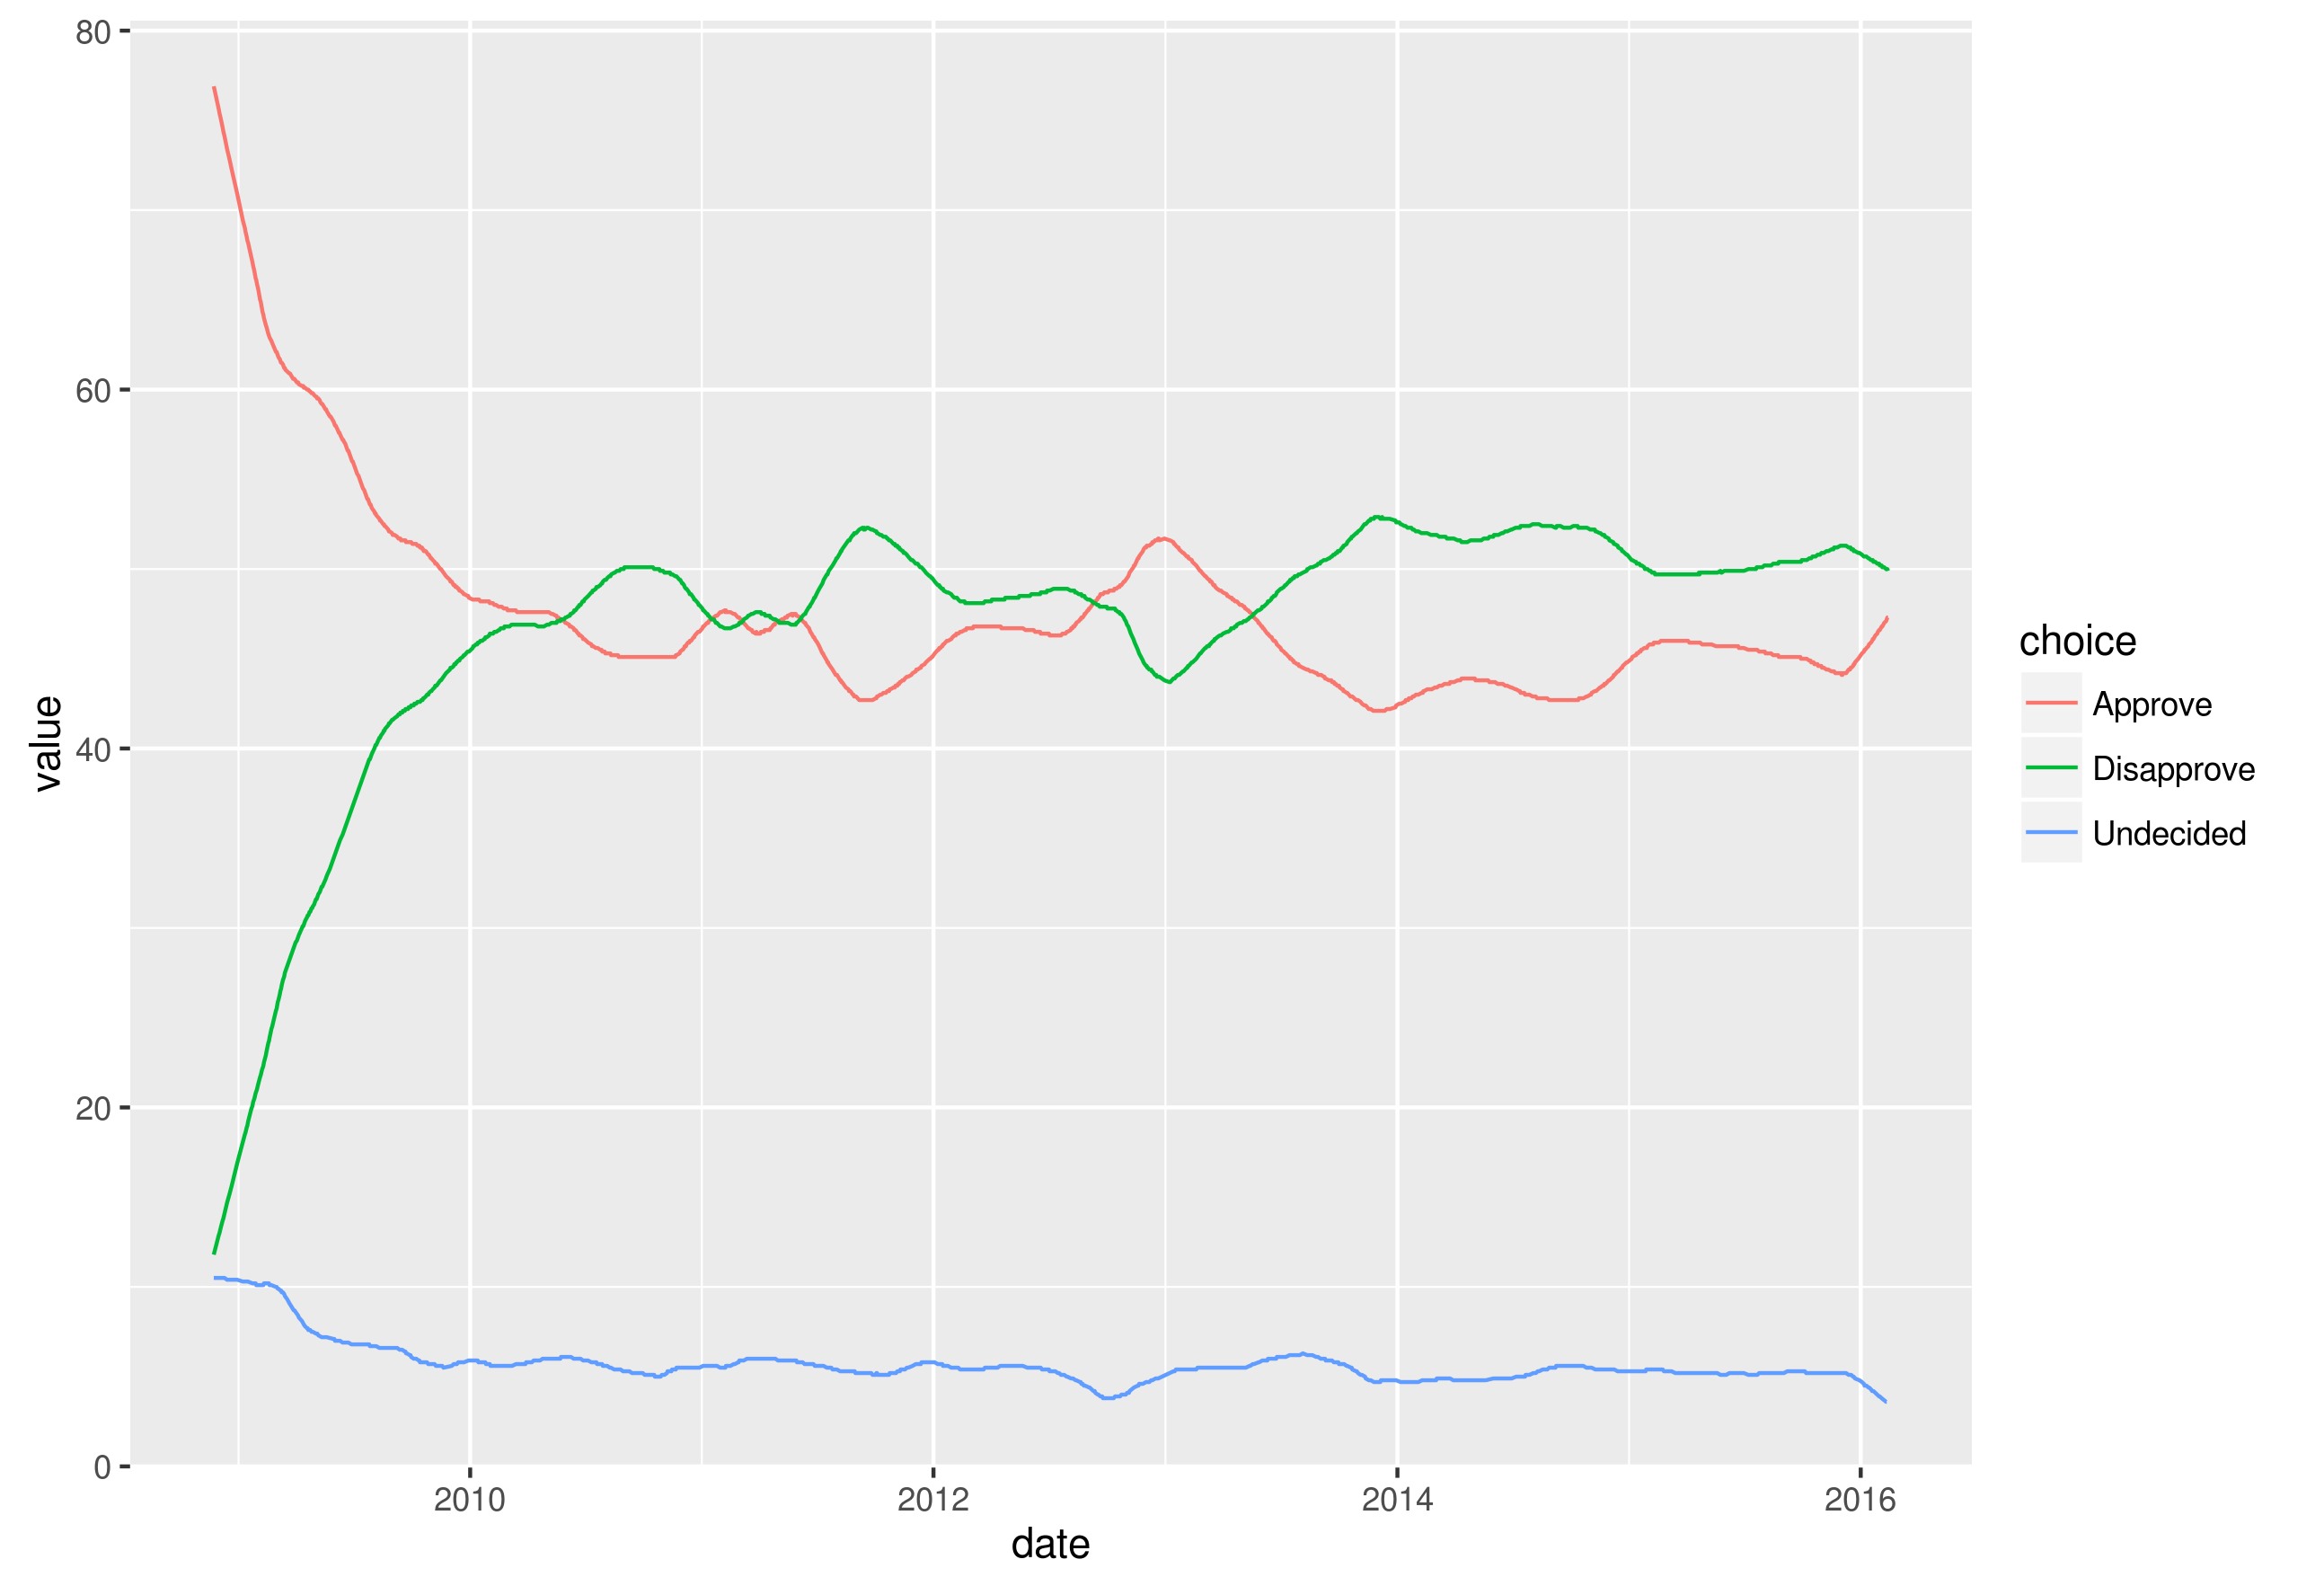
\includegraphics[width=\linewidth]{O_job_app.png}
\end{center}
\caption{Caption here}
\label{fig:figure4}
\end{figure}

From late 2008 the approval rate start high at about 80 percent, while the disapproval rate start as low as about 15 percent. The approval rate begin to decrease very fast whereas, oppositely the disapproval increased also at a fast rate until early 2010. From 2010 to now those have flatten at about 50 percent with some minor up and down.
\medspace

\item {\bf The Script}

The R Script used to produce this graph is shown bellow

\begin{lstlisting}[language = R]
# Creating the slug 
slug <- "obama-job-approval" 
# Create the chart using pollster library 
chart <- pollstr_chart(slug)
# Filter by date
estimates <- chart[["estimates_by_date"]]
# generate the plot using ggplt2
ggplot(estimates, 
          aes(x = date, y = value, color = choice)) + geom line()
# Save the image into the image directory as png file 
ggsave(file = paste(imageDirectory,"O_job_app.png",sep="/")) 
\end{lstlisting}

\end{enumerate}
 
\bigskip
\end{section}

\begin{section}
%\item % Congress Job approval
{\bf \large Congress Job Approval}
\begin{enumerate}[]
\item {} %  the chart

This chart bellow shows the American Congress job approval rating since the beginning of President Obama's presidency. In red is the approval rate and in green the disapproval rate.

\begin{figure}[htb]
\begin{center}
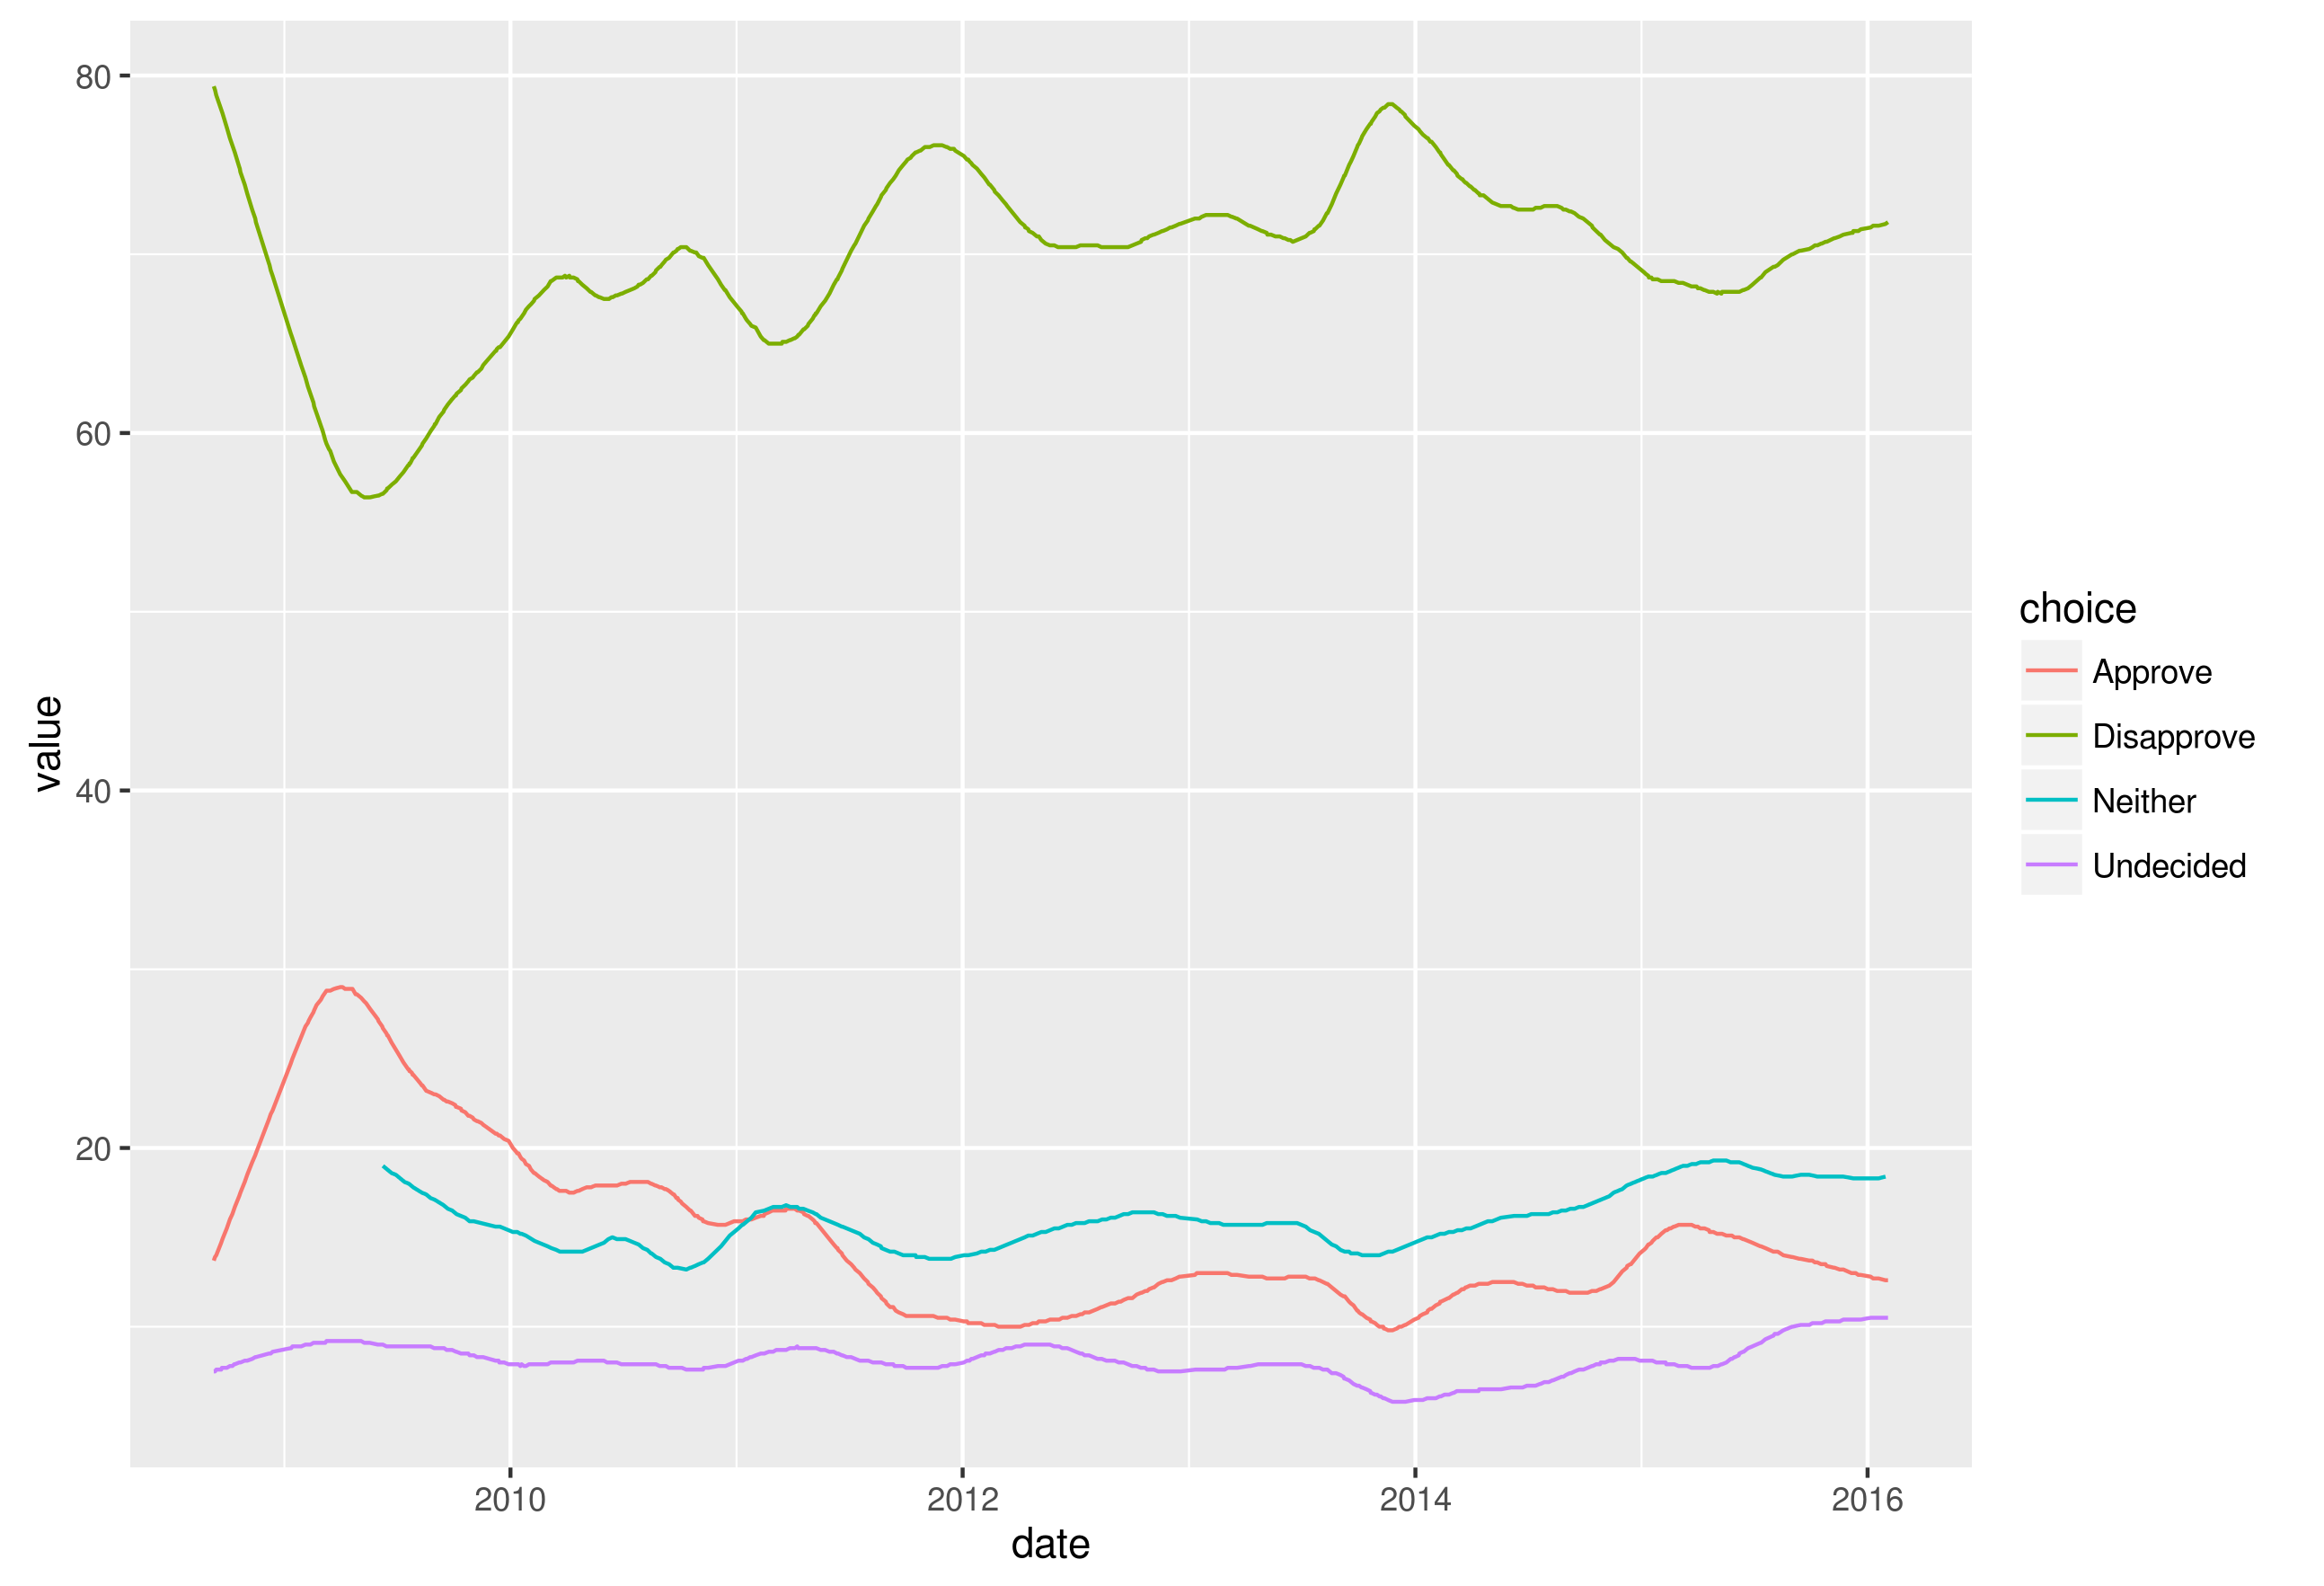
\includegraphics[width=\linewidth]{Congress_job_app.png}
\end{center}
\caption{Caption here}
\label{fig:figure 5}
\end{figure}

The analysis of this chart show that from late 2008 the disapproval rate was hight to around 80 percent while the approval rate was very low at about 15 percent. And the approval rate began increasing at a fast pace before attaining his pick at around 30 percent, whereas in the opposite  the disapproval rate started  rapidly decreasing  until attaining a minimal  value of about 55 percent. Then from  2009 to mid 2011 the approval and disapproval rate evolve at a lower pace in opposite direction with an increase of disapproval to truthfully 78 percent and a decrease of approval to around 12 percent. From there those rate have flatten until  now at about the 72 percent an 11 percent.

\item {\large {\bf The Script}}
\begin{lstlisting}[language = R]

slug <- "congress-job-approval"
## polster Chart
chart_congress <- pollstr_chart(slug)

# Filter by date
estimates_congress <- chart_congress[["estimates_by_date"]]

# Generate the plot using ggplot2 and save
ggplot(estimates_congress, 
               aes(x = date, y = value, color = choice)) + geom_line()
ggsave(file = paste(imageDirectory,"Congress_job_app.png",sep="/"))

\end{lstlisting}
\end{enumerate}

\end{section}


\end{document}